%%%%%%%%%%%%%%%%%%%%%%%%%%%%%%%%%%%%%%%%%%%%%%%%%%%
%
%  New template code for TAMU Theses and Dissertations starting Fall 2012.  
%  For more info about this template or the 
%  TAMU LaTeX User's Group, see http://www.howdy.me/.
%
%  Author: Wendy Lynn Turner 
%	 Version 1.0 
%  Last updated 8/5/2012
%
%%%%%%%%%%%%%%%%%%%%%%%%%%%%%%%%%%%%%%%%%%%%%%%%%%%
%%%%%%%%%%%%%%%%%%%%%%%%%%%%%%%%%%%%%%%%%%%%%%%%%%%%%%%%%%%%%%%%%%%%%%
%%                           SECTION V
%%%%%%%%%%%%%%%%%%%%%%%%%%%%%%%%%%%%%%%%%%%%%%%%%%%%%%%%%%%%%%%%%%%%%


\chapter{\uppercase{Experiments \& Results}}
To verify the idea proposed in this thesis, we setup environments, develop SAC framework and run some typical seismic applications on cluster in PVAMU cloud computing lab. There are three main layers in SAC: low-level runtime envrionment, SAC framework as middleware and application development interface at up-level. 

\section{Experiments Environment Setup}

The cluster used for conducting experiments consists of 26 nodes, in which one is management node, another is storage node used for managing disk array and other 24 nodes are computation nodes. Each node in such cluster was equipped with Intel Xeon E5-2640 Sandy Bridge CPU (2.5GHz, 12 Cores or 24 Cores with Hyperthreading support), 64GB DDR3 memory and are inter-connected with 1GB ethernet. Each node has its own local disk, and also could access disk array through NFS. Following the architecture stated in previous charpter, we install CentOS 6.5 (Distributed by Redhat) and Oracle JDK 1.8.0\_40 on each node. Hadoop 2.2.0, Spark 1.2.1 and other related libraries are also installed on each node. In configuration of Hadoop, management node was configured as NameNode and other 24 computation nodes as DataNodes. It is similiar in Spark: management node is Master and other computation nodes are Workers. Cassandra was installed on all 24 computation nodes and the first four nodes was selected as seed nodes.

The public sample seismic dataset Penobscot \cite{PenobscotData} was selected as experiment data. The original format of Penobscot dataset is SEGY, and to make it easily processed with Spark, we transfer it into two files: one xml file that saves meta data, and aonther 3D data file with dimension size of 600x481x1501 stores actual data samples. The volume size of original data file is about 1.7GB, which is not big enough comparing with data set currently used in oil\&gas industry, so we use it synthesize a new 100GB file for verifying algorithms and models on SAC. Both xml file and data file are stored on HDFS, so that every node could access them and utilize data locality. The intermediate results are stored in Cassandra basing on requirement and final result are persisted on HDFS. 

\section{Application Development Platform}

As stated in previous charpter, user could create new application that calls APIs provide by SAC framework, but another more convenient way is using Web interface provide by SAC platform. In web development interface, SAC platform provides four main components: Projects, Data Sets, Jobs and Workflow. The typical flow is listed below:

\begin{enumerate}
  \item Create a project or open an existing project. While create new project, user need to select template as shown in Figure \ref{NewProject}.
  \item Edit codes, compile project and fix erros until compiling successfully as shown in Figure \ref{Programming}.
  \item Select data set(s) as input parameter as shown in Figure \ref{DataSet}.
  \item Configure runtime environments and submit job to Spark Jobserver as shown in Figure \ref{Runtime}.
  \item Check job status and view results after job finished.
\end{enumerate}

%%%%%%%%%%%%%%%%%%%%%%%%%%%%%%%%%%%%%%%%%%%%%%%%%%%%%%%
\begin{figure}[H]
%\centering
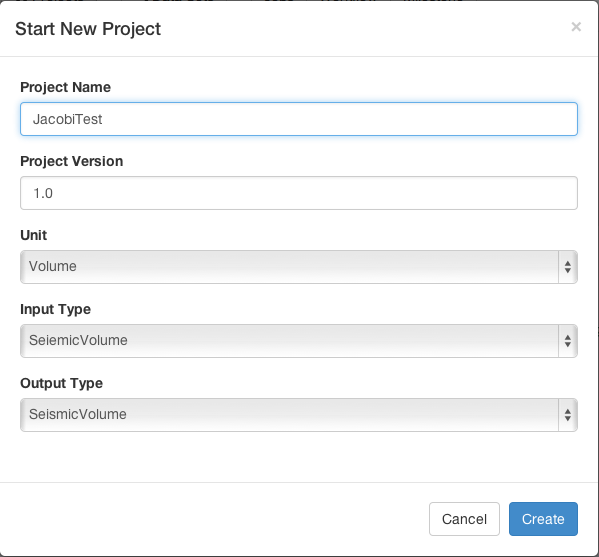
\includegraphics[scale=.60]{figures/NewProject.png}
\caption{Configure Template on Creating New Project}
\label{NewProject}
\end{figure}
%%%%%%%%%%%%%%%%%%%%%%%%%%%%%%%%%%%%%%%%%%%%%%%%%%%%%%%

%%%%%%%%%%%%%%%%%%%%%%%%%%%%%%%%%%%%%%%%%%%%%%%%%%%%%%%
\begin{figure}[H]
\centering
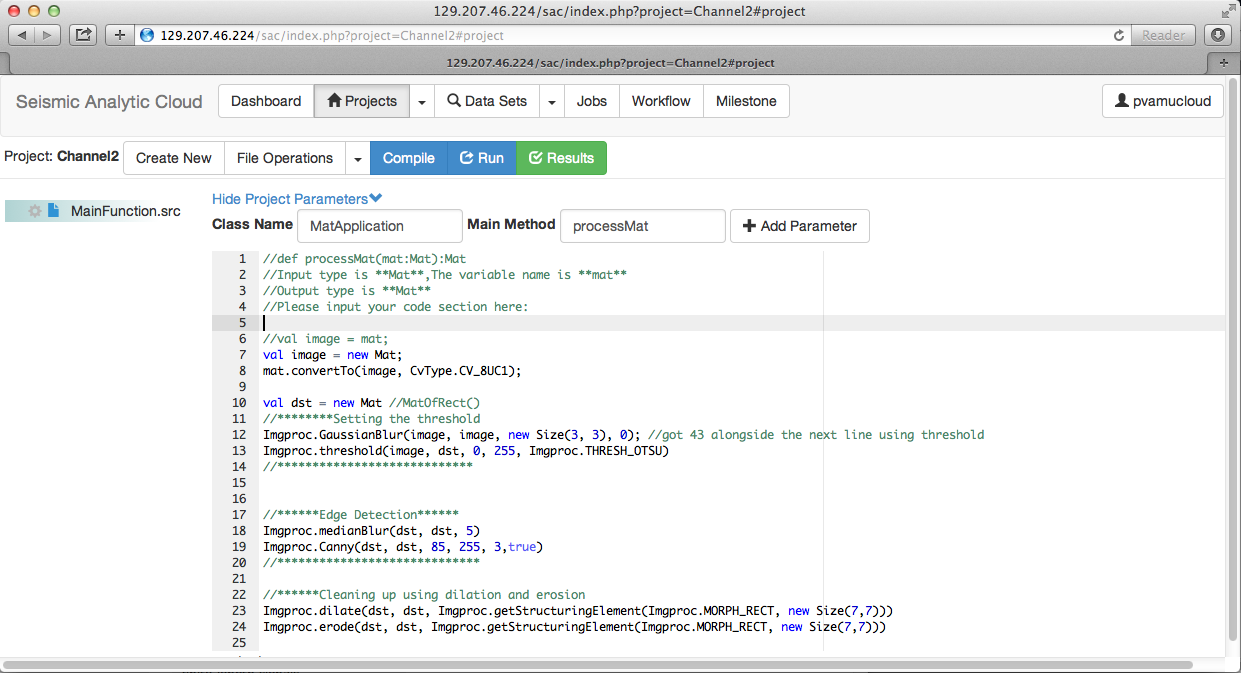
\includegraphics[scale=.35]{figures/Programming.png}
\caption{Programming and Running on Web Interface}
\label{Programming}
\end{figure}
%%%%%%%%%%%%%%%%%%%%%%%%%%%%%%%%%%%%%%%%%%%%%%%%%%%%%%%


%%%%%%%%%%%%%%%%%%%%%%%%%%%%%%%%%%%%%%%%%%%%%%%%%%%%%%%
\begin{figure}[H]
\centering
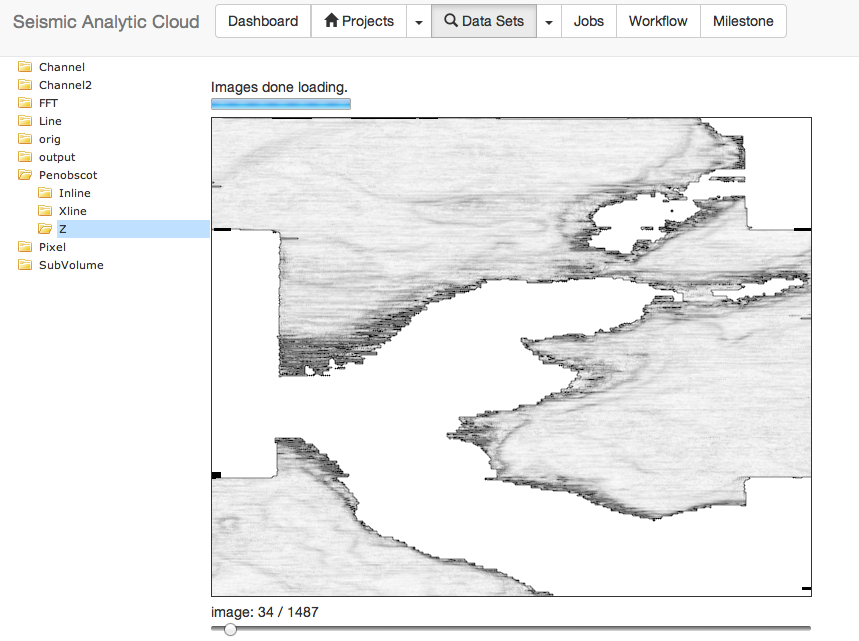
\includegraphics[scale=.45]{figures/DataSet.png}
\caption{Seismic Dataset Preview}
\label{DataSet}
\end{figure}
%%%%%%%%%%%%%%%%%%%%%%%%%%%%%%%%%%%%%%%%%%%%%%%%%%%%%%

%%%%%%%%%%%%%%%%%%%%%%%%%%%%%%%%%%%%%%%%%%%%%%%%%%%%%%%
\begin{figure}[H]
\centering
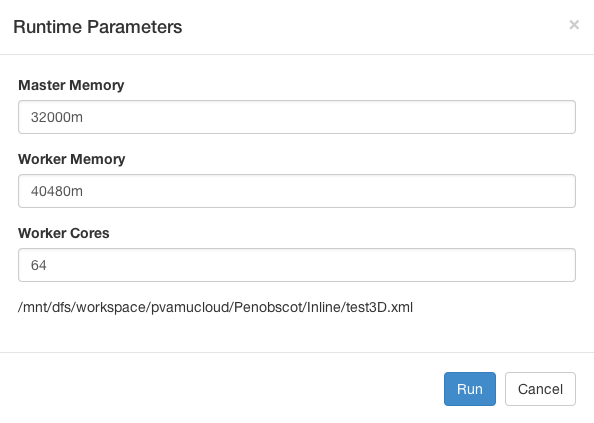
\includegraphics[scale=.60]{figures/Runtime.png}
\caption{Specify runtime parameters}
\label{Runtime}
\end{figure}
%%%%%%%%%%%%%%%%%%%%%%%%%%%%%%%%%%%%%%%%%%%%%%%%%%%%%%

%A table example is going to follow.
\begin{table}[H]
\centering
\caption{Provided UFuncs by ScalaNLP Breeze}
%\begin{tabular}{|p{4cm} |p{8cm} |}
\begin{tabular}{|l|l|}
\hline
Elementwise UFuncs & \shortstack[l]{exp, log, log1p, sqrt, \\sin, cos, tan, asin, acos, atan,\\sinh, cosh, tanh, asinh, acosh, atanh, \\floor, ceil, round, rint, signum, \\abs, isOdd, isEven,sigmoid} \\ 
\hline
Operator UFuncs &  \shortstack[l]{OpAdd: a + b, OpSub: a - b, OpMulMatrix: a * b, \\OpMulScalar: a :* b, OpSolveMatrixBy: a \textbackslash b,\\ OpMulInner: a dot b, OpNeg: -a, OpEq: a :== b, OpNe: a:!= b, \\ OpLT: a:\textless b, OpLTE: a :\textless= b, OpGT: a :\textgreater b, OpGTE: a :\textgreater= b, \\OpAnd: a \& b, OpOr: a \textbar b, OpNot: !a } \\
\hline
Reduction UFuncs & \shortstack[l]{sum, product, softmax, any, all, \\min, max, argmin, argmax, \\norm, normalize, argsort, argtopk, \\mean, variance, stddev, meanAndVariance }\\
\hline
\end{tabular}
\label{tab:BreezeUFuncs}
\end{table}
%%%%%%%%%%%%%%%%%%%%%%%%%%%%%%%%%%%%%%%%%%%%%%%%%%%%%%

\section{Case Study}
The main characteristics of SAC are productivity, performance, usability and scalability. To prove them, some typical applications in seismic data processing are selected to run on SAC. As for usability and productivity, we will show some codes snippet need to be implemented by end user. As for the performance, executation time of both sequential codes and parallel codes on Spark are compared to get speedup factor, and for scalability, we will configure the running environment with different cores and analyse changing of executation time. To cover more seismic applications, we select four applications as test cases: Calculactor, Transformation, Statistics Functions and Jacobi Stencil codes.

\subsection{Calculactor}
Calculactor should be the most common used tool in scientific computation. Basic arithmetic operations are easy implemented on normal data, but for big data, the situation is totally different. There are already some commerical and free seismic calculators such as Calculactor in Petrel, Seismic Toolkit listed in \cite{SeismicCalculator} etc. All these seismic calculator are software running on PC, so the performance is bad for handling big seismic data, and most of them even could handle big data. Calculactor designed in SAC is mainly focus on handling big data, in which data is distributed on different nodes and run arithmetic functions in parallel. Most functions in calculator are applied on pixel or sample, and each pixel is a Float type in Scala, so all built-in operator could be used on pixel data. The more convenient way to implement such algorithms are use operators and operations provided by Breeze. For trace or line template in SAC, the data types of input and output are DenseVector and DenseMatrix. ScalaNLP Breeze provide many Universal Functions (UFunc) that can operate on scalars, vectors, matrices, counters with little effort \cite{BreezeUFunc}. All Elementwise UFuncs from scala.math such as exp, log and trigonometric functions etc., and Operator UFuncs such as basic Arighmetic, equality and comparison and boolean operations could be applied to DenseVector and DenseMatrix.   


\subsection{Filter \& Transformation}

\subsection{Statistics functions}

\subsection{Complicate Stencil Operation}





